\subsection{Convolutional Neural Networks}
  Convolutional Neural networks(CNN) have been prominent in the field of Computer vision in recent years.
  Computer vision uses CNNs to classify images with high accuracy and speed \cite{razavian2014}.
  CNNs come at the cost of requiring long times to train, in most cases using GPUs \cite{krizhevsky2012}.
  Therefore, the standard use of CNNs is impractical for tracking unknown objects; training a CNN online impairs the system's speed \cite{bertinetto2016}.

  \subsubsection{Crowd Segmentation with CNNs}
  A crucial part of tracking is distinguishing background from objects of interest.
  \citet{kang2014} propose fast fully-convolutional neural networks(FCNN) to segment crowds.
  Fully convolutional means that the CNN is invariant under the translation of the input image.
  The FCNN searches a whole image in one pass of forward propagation through the network.
  This process allows faster and more accurate segmentation compared to sliding window techniques.

  The CNN of FCNN has no fully connected layers; instead, it uses a $1 \times 1$ convolution kernel layer to predict labels.
  This design removes the translation dependence, due to fully connected layers, from the network.
  The translation invariance of the network allows it to search a whole image in one pass.

  The FCNN uses appearance to segment the crowd--reducing the false positives occurring in motion cue segmentation.
  Another advantage of scanning the whole input image at once is the availability of more contextual appearance information, which aids the segmentation \cite{eigenFacesRecog, farabet2012}.
  Once an image of a crowd is segmented, another system can do a more specific analysis, such as identifying people.

  \subsubsection{Multi-domain CNN}
  \citet{CNNTracking} use a CNN as the basis of their tracker(MDNet). 
  MDNet trains on a large, labelled dataset of videos to obtain generic target representations.
  The CNN learns one domain, cars say, at a time; all the domains are worked through iteratively.
  This process provides a CNN that can distinguish between any target and background in the trained domains.

  \begin{figure}[!ht]
    \centering
    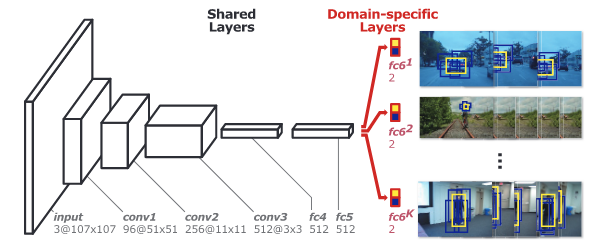
\includegraphics[scale=0.5]{MDNet.png}
    \caption{The architecture of the Multi-Domain Network, from \protect\cite{CNNTracking}}
    \label{fig:mdnet}
  \end{figure}
  The output of this CNN branches into input for domain-specific layers see Figure~\ref{fig:mdnet}.
  These output layers are binary classifiers that use the network's generic representation to track a target in a specific domain.
  These classifiers use the video stream as input to improve the tracker's accuracy by learning online.

  This design allowed \citeauthor{CNNTracking} to get very high accuracy in VOT challenges.
  The high accuracy comes at the cost of real-time execution--the binary classifiers of the network require a lot of time to train online.
  MDNet was only able to process one frame per second in the VOT challenges \cite{bertinetto2016}--making it unsuitable for real-time tracking.
  

  \subsubsection{Convolutional Siamese Neural Networks}
  \citet{bertinetto2016} offer another method of tracking an unknown object with Convolutional Neural networks.
  The method given by \citeauthor{bertinetto2016} is to train, offline, a CNN that solves the more general similarity problem.
  Their system learns a similarity function $f(z,x)$ that compares the images $x$ and $z$; The system produces values that estimate how similar the images are.
  This function is equivalent to a composition of two other mappings: $f(z, x) = g(\phi(z), \phi(x))$.
  This composition consists of an embedding, $\phi$,  that does the convolution and a metric, $g$ .
  A siamese neural network, two identical neural networks conjoined at the output node \cite{bromley1993}, is used to learn the similarity relation.

  \citeauthor{bertinetto2016} suggest a \textit{fully-convolutional} siamese network to learn the similarity relation.
  The input to the network is an image centred on the target's previous location.
  The network outputs a score map represented as a grid of numbers, Figure~\ref{fig:convSiamese}.

  \begin{figure}[!ht]
    \centering
    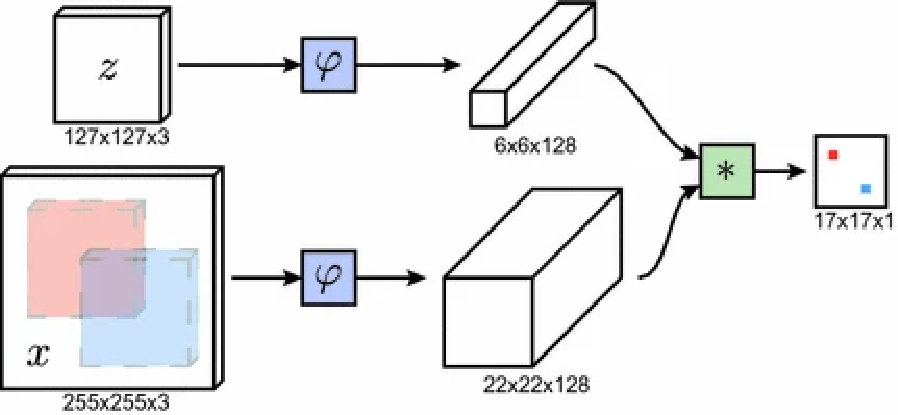
\includegraphics[scale = 0.6]{convSiamese.pdf}
    \caption{The architecture of the Fully Convolutional Siamese Neural Network, from \protect\cite{bertinetto2016}}
    \label{fig:convSiamese}
  \end{figure}

  This architecture is in the form of an advanced template tracker.
  The CNN is equivalent to the preprocessing needed to create a tracking template.
  The metric $g$ compares the template and a search window--often, template trackers use the sum of squares metric \cite{templateUpdate}.

